\documentclass{beamer}

\usepackage[utf8]{inputenc}
\usepackage[english]{babel}
\usepackage{graphicx,hyperref,ru,url}
\usepackage{multirow}
\usepackage[absolute,overlay]{textpos}

% The title of the presentation:
%  - first a short version which is visible at the bottom of each slide;
%  - second the full title shown on the title slide;
\title[ENSIAS - Business Intelligence]{
  Analyse de la concurrence du Groupe OCP sur le marché des phosphates et produits dérivés}

% Optional: a subtitle to be dispalyed on the title slide
\subtitle{\tiny{Soutenance Priliminaire PFE}}

% The author(s) of the presentation:
%  - again first a short version to be displayed at the bottom;
%  - next the full list of authors, which may include contact information;
\author[SEFIANE \& YACHAOUI]{
  Hamza SEFIANE \& Ayman YACHAOUI \\\medskip
  {\small \textbf{Encadrés par} : M. Ibrahim AMRANI} \\ 
  {\small \textbf{Jugés par} : Said ACHCHAB}}

% The institute:
%  - to start the name of the university as displayed on the top of each slide
%    this can be adjusted such that you can also create a Dutch version
%  - next the institute information as displayed on the title slide
\institute[]{
  École Nationale Supérieure d'Informatique et d'Analyse des Systèmes}

% Add a date and possibly the name of the event to the slides
%  - again first a short version to be shown at the bottom of each slide
%  - second the full date and event name for the title slide
\date[Année universitaire 2015-2016]{
  Mercredi 11 Mai 2016}

\begin{document}

\begin{frame}
  \titlepage
\end{frame}

\begin{frame}
  \frametitle{Outline}

  \tableofcontents
\end{frame}

% Section titles are shown in at the top of the slides with the current section 
% highlighted. Note that the number of sections determines the size of the top 
% bar, and hence the university name and logo. If you do not add any sections 
% they will not be visible.
\section{Introduction}


\begin{frame}
  \frametitle{Introduction}

  \begin{itemize}
    \item Presque toutes les décisions prises par un gestionnaire ont besoin d'une prévision.
    %\item Il a également besoin d'évaluer l'effet de ses décisions actuelles sur l'avenir afin que les bonnes décisions soient prises aujourd'hui pour créer une condition souhaitée demain.
    \item Optimisation des mouvements de stock, de cash-flows et régimes de production.
    \item Augmenter les ventes et améliorer les profits.
  \end{itemize}
\end{frame}

\section{Contexte Général}

\begin{frame}
	\begin{center}
		\Huge \textbf{\textit{Contexte Général}}
	\end{center}
\end{frame}

\begin{frame}
	\frametitle{Organisme d’accueil}
	\begin{textblock*}{7cm}(1cm,3cm)
		\begin{itemize}
			\item Fondé le 7 août 1920 au Maroc.
			\item L'un des principaux exportateurs de phosphate brut, d’acide phosphorique et d’engrais phosphatés dans le monde.
			\item 4 sites miniers et 2 complexes chimiques, ainsi que sur d'autres sites internationaux.
		\end{itemize}
	\end{textblock*}
	
	\begin{textblock*}{5cm}(9cm,3.5cm) % {block width} (coords)
		
\includegraphics[width=2.5cm]{logo-ocp}
	\end{textblock*}
\end{frame}

\begin{frame}
\frametitle{Situation Actuelle}
\begin{block}{L'OCP}
\begin{table}
\centering 
  \begin{tabular}{|c|c|c|c|}
  \hline
  \small{Produit} & \small{Capacité A.} & \small{PdM Internationale} & \small{Position} \\
  \hline
  Roche & 28.1 & 37\% & Leader\\
  MGA & 4.4 & 52\% & Leader\\
  Fertilisants & 4.35 & 16.5\% & 3e\\
  \hline
  \end{tabular}
  \end{table}
  \begin{itemize}
  \item Devenir un leader des coûts.
  \item	Contrôler la valeur de la roche.
  \item Veiller sur le marché.
  \end{itemize}
  \end{block} 
\end{frame}

\begin{frame}
  \frametitle{Motivation}
  \begin{block}{Motiver une prévision de la demande internationale}
    \begin{itemize}
    \item La demande d'engrais dépend d'une variété de facteurs agro-économiques.
    \item Tirer pleinement parti des fluctuations des cours mondiaux du marché. %Le stockage requis, le transport, les ressources humaines à mobiliser, les arrangements financiers de crédits et de devises étrangères sont tributaires de la demande.
    \item  Répondre aux questions $\rightarrow$ quant à quoi, quand et combien produire.
    \end{itemize}
    \end{block}
\end{frame}

\section{Analyse}

\begin{frame}
	\begin{center}
		\Huge \textbf{\textit{Analyse}}
	\end{center}
\end{frame}

\begin{frame}
  \frametitle{Méthodes de Prévision}
  \begin{block}{Etapes}
  \small{La prévision de la consommation en fertilisants peut être décomposées en 3 étapes complémentaires.
  \begin{enumerate}
  \item Evaluation du potentiel.
  \item Prévision de la demande.
  \item Prévision des ventes.
  \end{enumerate}
  }\end{block}
\end{frame}
\begin{frame}
  \frametitle{Méthodes de Prévision}
	\begin{block}{Approches Possibles}
	\small{
	\begin{itemize}
	\item Méthodes agronomiques (orientées besoin).
	\item Analyse des séries chronologiques et projections.
	\item Analyse causale.
	\item Approche qualititative.
	\end{itemize}
	}
	\end{block}
\end{frame}

	\begin{frame}
	\frametitle{Les critères du choix}
	
	\begin{block}{Choisir l'approche}
	Le but de prévision $ \in $ \footnotesize{ [ Besoin immédiat logistique , Décisions long-terme ] }
	 \\
	\begin{block}{}
	\small{Dans le court-terme, le passé pèse plus sensiblement : \\ $\rightarrow$  L'approche SC est adaptée pour les besoins court/moyen terme.}
		\end{block}
		\end{block}

	\end{frame}
	\begin{frame}
	\frametitle{L'Approche adoptée}
	
	\begin{block}{Analyse SC \& Projections}
	\begin{itemize}
	\item Les données historiques en fertilisants sont compilées.
	\item Ces données sont décomposées en tendance, cycle, saisonnalité et résidus aléatoires 
	\item Plusieurs modèles SC sont testés et comparés sur des données de Test.
	\end{itemize}
	\end{block}
	\end{frame}
\begin{frame}
\frametitle{Besoin d'une banque de Données}
\begin{block}{}
\footnotesize{L'efficacité d'une prévision de la demande comme un outil de décision dépend de la disponibilité de données sur les surface arables, prix des fertilisants, sensibilité des récoltes aux fertilisants, consommation historiques, etc.}
\center{
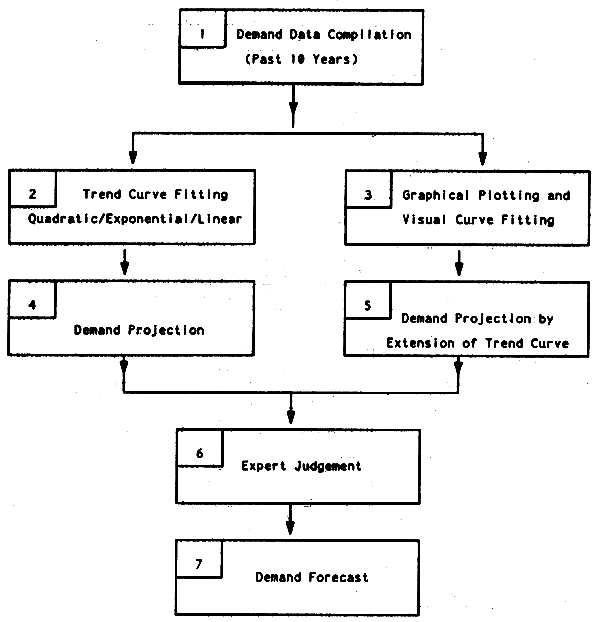
\includegraphics[width=0.6\textwidth>,height=0.6\textheight]{TS_WF}}

\end{block}
\end{frame}
\section{Réalisation}

\begin{frame}
	\begin{center}
		\Huge \textbf{\textit{Réalisation}}
	\end{center}
\end{frame}

\begin{frame}
  \frametitle{Collecte de données}
  \textbf{La collecte et la préparation de données} représentent \textbf{80\%} d'un projet d'analyse de données.\\
  \begin{itemize}
    \item Documents cible : Des PDFs contenant des Trades Matrix concernant differents produits Phosphaté.
    \item Données cible. : Les Imports et Exports régionaux de ces différents produits.
  \end{itemize}
\end{frame}

\begin{frame}
  \frametitle{Collecte de données}
	\begin{block}{Document cible}
    		\begin{center}
    		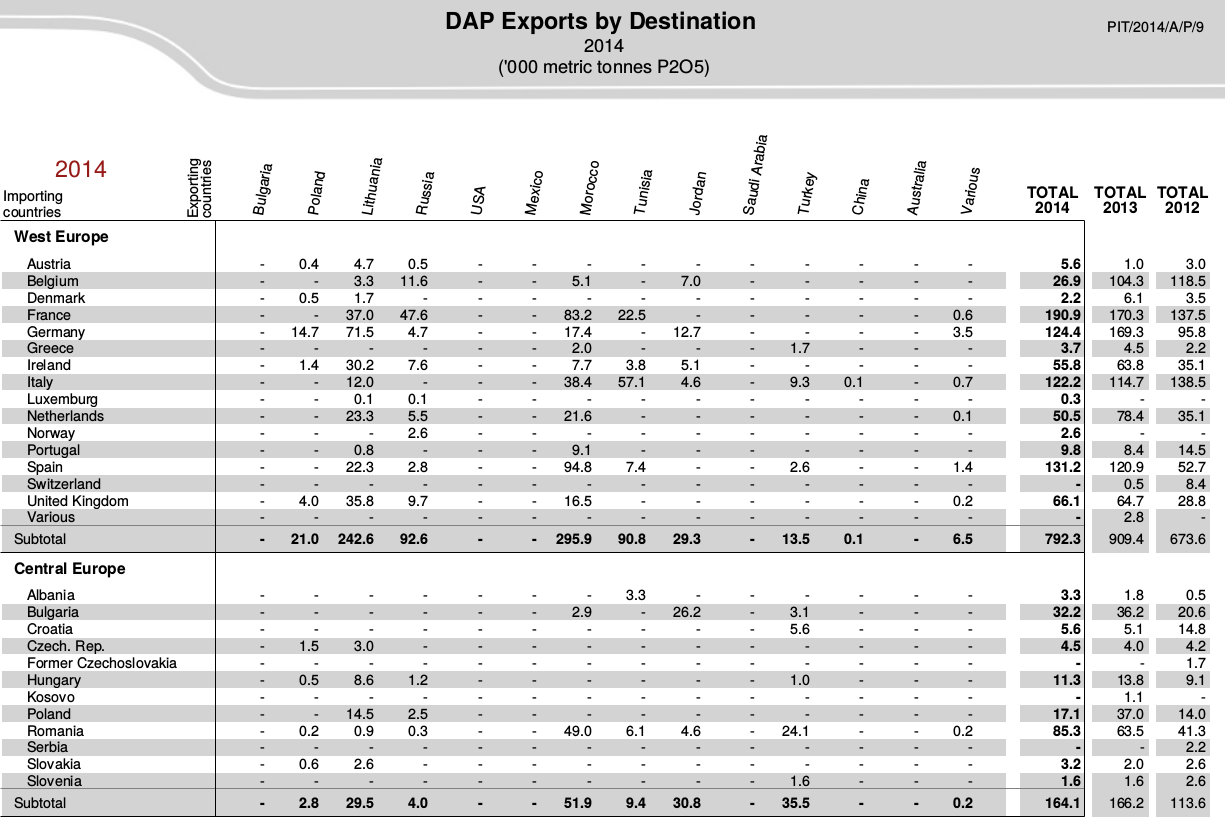
\includegraphics[width=\textwidth, height=0.7\textheight, keepaspectratio]{DocIFA}
    		\end{center}
	\end{block}
\end{frame}

\begin{frame}
  \frametitle{Collecte de données}
  \framesubtitle{\textbf{\textcolor{yellow}{Contrainte}}}
  \begin{block}{contrainte}
  	\begin{itemize}
    		\item Le document ne contient pas que des Trades Matrix.
    		\item Trade Matrix de quel produit ?
    		\item Pas évident d'extraire la structure d'une table dans un PDF.
  	\end{itemize}
  \end{block}
\end{frame}

\begin{frame}
  \frametitle{Collecte de données}
  \framesubtitle{\textbf{\textcolor{yellow}{Méthodologie}}}
	\begin{block}{WorkFlow}
% Your image included here
    		\begin{center}
    		\includegraphics[width=\textwidth, height=0.7\textheight, keepaspectratio]{IFAParser}
    		\end{center}
	\end{block}
\end{frame}


\begin{frame}
  \frametitle{Collecte de données}
  \framesubtitle{\textbf{\textcolor{yellow}{Méthodologie}}}

  \begin{block}{Outils}
  	\begin{itemize}
    		\item Language : Python, Bash.
    		\item Packages : PdfTable, RegEx, csv.
  	\end{itemize}
  		
\includegraphics[width=4cm]{python}
  		\hspace{2cm}
		
\includegraphics[width=1.6cm]{Bash}
		
  \end{block}
 \end{frame}
 
 \begin{frame}
  \frametitle{Collecte de données}
  \framesubtitle{\textbf{\textcolor{yellow}{Résultat}}}

    Requêtage simple pour extraire les différentes quantité échangée pour un pays ou une région donnée.\vspace{1mm}
	\begin{center}
	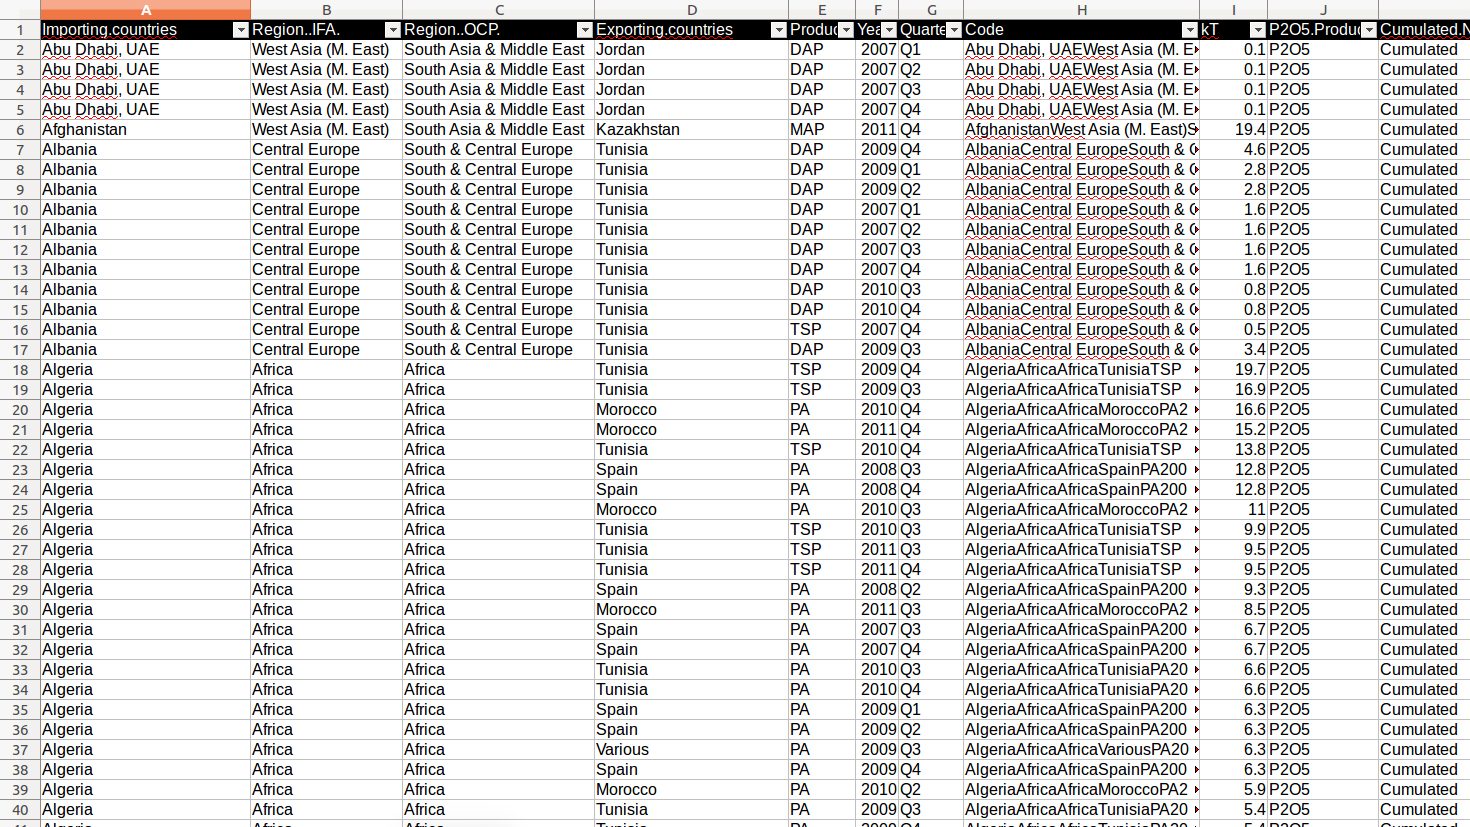
\includegraphics[width=0.8\textwidth, height=0.7\textheight, keepaspectratio]{IFAcsv}
	\end{center}
  
 \end{frame}

\section{Conclusion}


\begin{frame}
  \frametitle{Conclusion}

  \begin{itemize}
    \item [PS] – SARIMA
    \item [AS] – SARIMA
    \item [AS(R)] – SARIMA
  \center{
  Merci pour votre attention.}
  \end{itemize}
\end{frame}

\end{document}
